% !TeX spellcheck = en_US


\chapter{Introduction}


\section{Biological Whiskers}

In modern robotics touch is often neglected in favor of vision for navigation and object recognition~\cite{s22072705}.
However, vision is often limited by light conditions and occlusions.
Many animals, such as cats or rats, have developed a tactile sensing system based on vibrissae (whiskers), that complement their vision.
The anatomical structure of the whiskers is shown in Figure~\ref{fig:whisker-anatomy}.

\begin{figure}[htb]
    \centering
    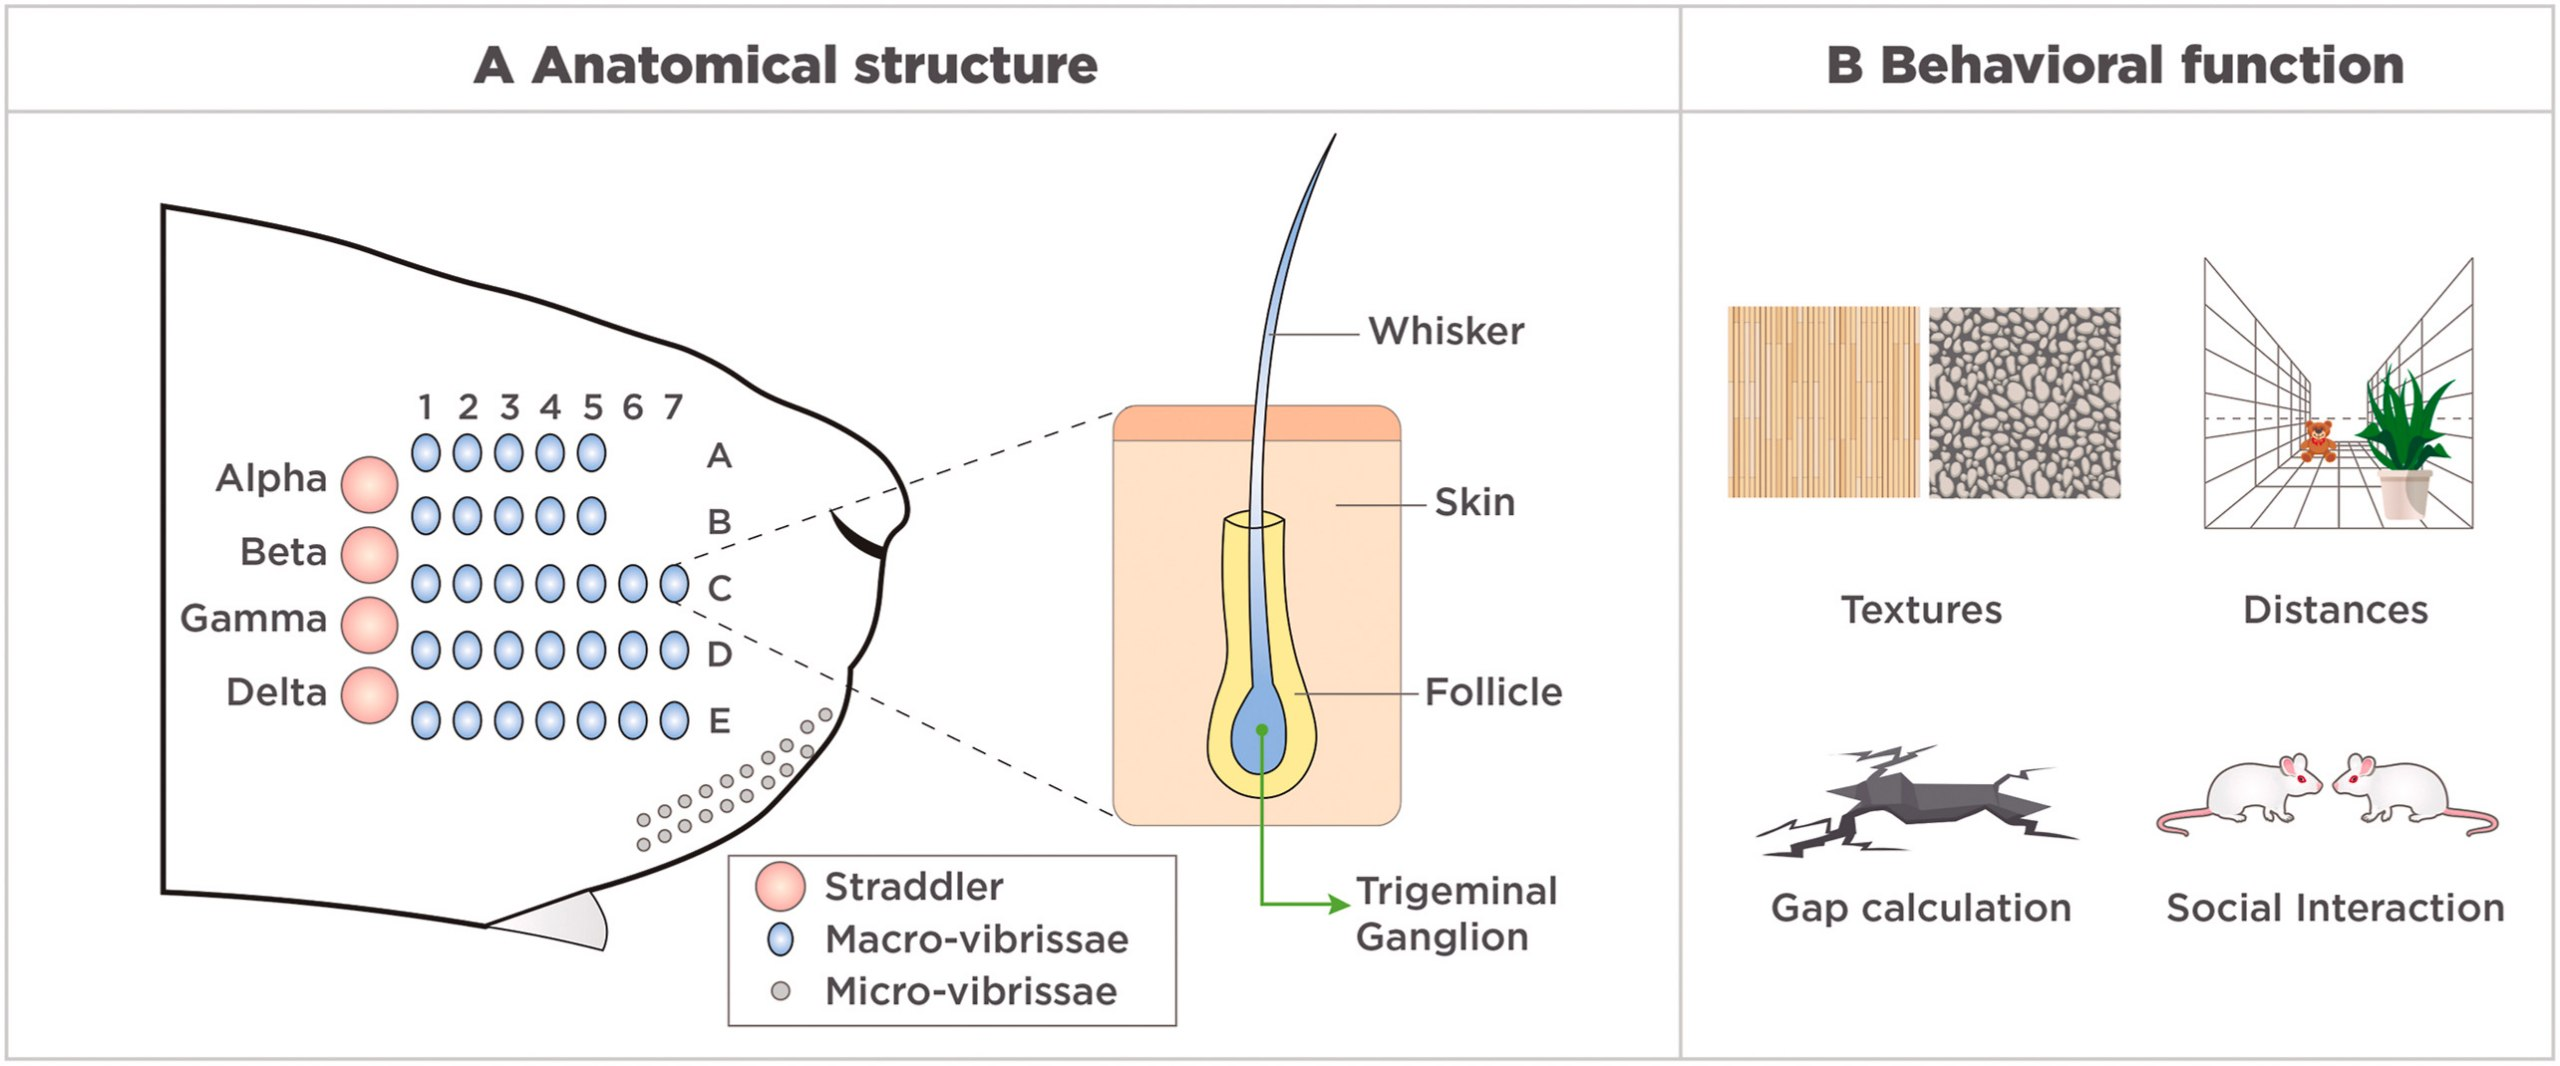
\includegraphics[width=\textwidth]{figures/whisker-anatomy}
    \caption{Representation of the vibrissae system and its function, from~\cite{IBARRACASTANEDA2022100034}}
    \label{fig:whisker-anatomy}
\end{figure}

For example, seals and sea lions use their whiskers in dark and turbid waters during hunting.
When the prey passes the animal, vortices are created and whiskers are deflected in a jerky motion, exposing the hydrodynamic trail of the prey~\cite{muthuramalingam2018sealsealionwhiskers}.
While seals and sea lions use their whiskers passively, other animals like rats and squirrels adopted active whisking motions to explore their environment.
For instance, whisking allows them to discriminate texture of the objects as different textures produce different magnitude and temporal pattern of slip-stick motion, which causes transient resonance in the whiskers~\cite{wolfe2008texture}.
Some nocturnal species primarily rely on their whiskers instead of vision.


\section{Robotic Whisker Sensors}

This versatility of the whiskers serves as an inspiration for the development of robotic whisker sensors.
They are particularly advantageous for SLAM of cluttered unstructured environments, where vision is limited and mobility is restricted.
Whiskers can help avoid obstacles and precisely reconstruct object contours.
Another benefit of whiskers over vision in that regard is their low computational requirements, high spatial resolution and lightweight design.
Robotic whisker sensors employ different sensing modalities, such as strain gauges, Hall effect sensors or optical sensors to measure the deflection of the whisker.
Taxonomy of whisker sensors is shown in Figure~\ref{fig:taxonomy}.
Optical setups are usually bulky, complex and expensive as they require a camera.
Strain gauges are small and cheap, but they are very temperature sensitive and require precise calibration~\cite{s19214713}.
In this work we opt for the Hall effect sensor, which is small, cheap and easy to integrate into a whisker sensor.

While whisker sensors are able to detect the contact point by measuring the deflection, caused by the contact forces, active control is required to reconstruct the contour of the object.
Furthermore, a contour tracking algorithm is needed to reconstruct the object shape without the gaps.
While several studies focused on basic contour tracking algorithms, such as the one proposed by~\cite{lin2022whiskerinspiredtactilesensingcontact}, they are not robust to sharp corners and do not consider the whisker detachment.

\begin{figure}[htb]
    \centering
    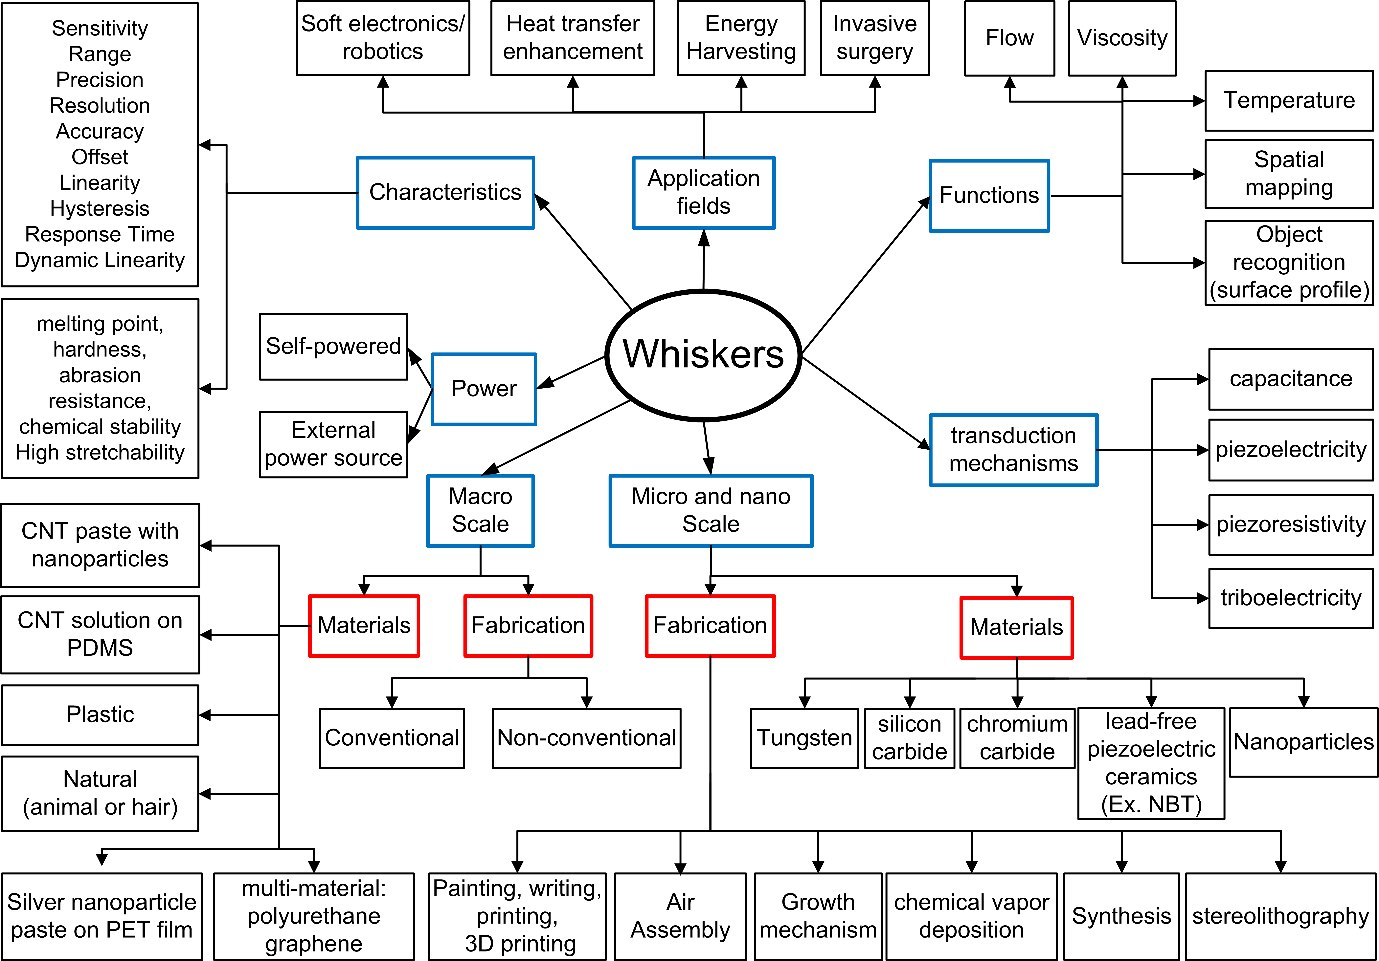
\includegraphics[width=0.65\textheight]{figures/taxonomy}
    \caption{A taxonomy for whisker-based sensors, from \cite{s22072705}}
    \label{fig:taxonomy}
\end{figure}

\section{Key Contributions}

\begin{enumerate}
    \item We present a new \textbf{whisker sensor array} design using magnetically transduced whiskers, with 3 whiskers on each side of the platform.
    \item We introduce \textbf{Swiping policy} for uninterrupted contour tracking, achieving a submillimeter accuracy.
    It balances between preserving optimal whisker deflection and following the object's surface tangentially.
    \item We propose \textbf{Retrieval policy} for object retrieval in case of whisker detachment at sharp corners, managing the entire range of corner angles and ensuring edge contour reconstruction.
    It involves edge angle resolution, whisking back and reattaching the whisker to the object.
    \item We develop a \textbf{Tunneling policy}, allowing navigation in tunnels, for multi-whisker setups and show that it is able to maintain a centered trajectory in confined passages.
    It aims to keep the whiskers in contact with the walls, while following the tunnel and avoiding collisions.
    \item Additionally, we prepare a \textbf{simulation framework} for the whisker control system to automate the testing of the control policies.
    MuJoCo physics engine is used to simulate the whisker sensor and the environment.
    \item Finally, we present a \textbf{system infrastructure} for real-time sensor data visualization and evaluation.
    It is designed to be modular and extensible, and provides functionality for active control, data collection, storage and visualization.
\end{enumerate}
